\documentclass{../exhibit}


%% Ben Szczesny and
%% Bart Snapp


\title{Number Mazes}

%% Font
\usepackage{imfellEnglish}
\usepackage[T1]{fontenc}
\raggedright

\usepackage[LGRgreek]{mathastext}


%% so title is accessable
\makeatletter
\let\thetitle\@title
\let\theabstract\@abstract
\makeatother


\usepackage{background}
\backgroundsetup{
scale=1,
color=white,
opacity=0.2,
angle=0,
contents={%
  \hspace{0 in}\raisebox{0 in}{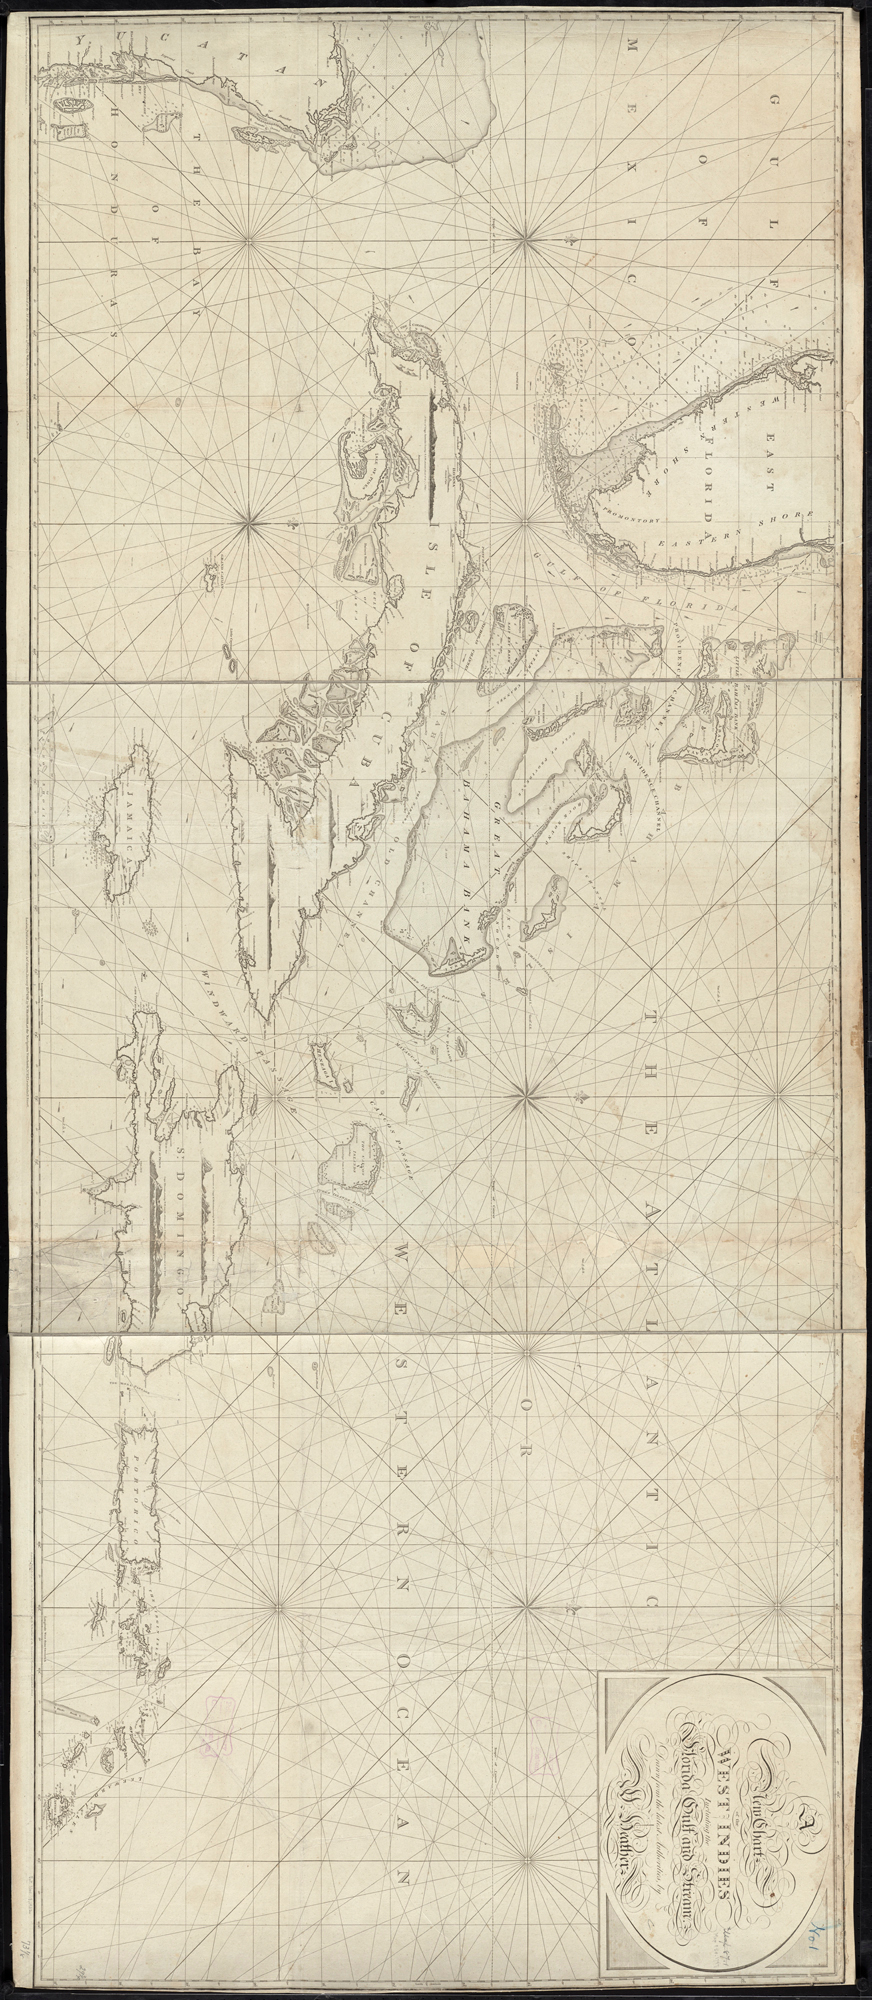
\includegraphics[scale=.5]{mapBackground.jpg}}
  %%https://commons.wikimedia.org/wiki/File:1683_Mortier_Map_of_North_America,_the_West_Indies,_and_the_Atlantic_Ocean_-_Geographicus_-_Atlantique-mortier-1693.jpg
  }%
}


\def\imagetop#1{\vtop{\null\hbox{#1}}}

%% For the context
%% https://tex.stackexchange.com/questions/86150/torn-page-effect/86151#86151
\usepackage{tikz}
\usetikzlibrary{decorations.pathmorphing}
\definecolor{paper}{RGB}{239,227,157}


%% QR code
\usepackage{qrcode}



%% For bold-ish title
\usepackage{shadowtext}



\renewcommand{\maketitle}{ %
  \shadowoffset{.5pt} %% See: https://tex.stackexchange.com/questions/159463/fancy-styled-borders-in-latex
  \shadowcolor{black!50!white}
  \begin{center}
    \resizebox{\textwidth}{!}{\shadowtext{\scshape\thetitle}}
  \end{center}
  
\vspace{1cm}
  
\begin{tabular*}{\textwidth}{c @{\extracolsep{\fill}} c}  
  \imagetop{
\begin{tikzpicture}
        \node[preaction={fill=white,opacity=0},inner sep=.5cm] 
             {
               \begin{minipage}{.45\textwidth}\Huge\directions\end{minipage}
             };
  \end{tikzpicture}}
  &
  \imagetop{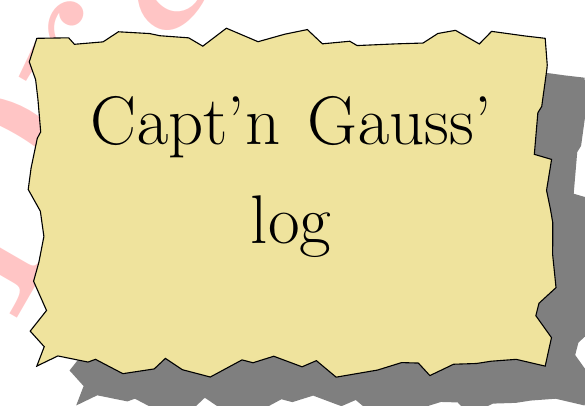
\begin{tikzpicture}[pencildraw/.style={ %%% https://tex.stackexchange.com/questions/86150/torn-page-effect/86151#86151
            decorate,
            decoration={random steps,segment length=8pt,amplitude=4pt}
          } %
        ]
        \node[preaction={fill=black,opacity=.5,transform canvas={xshift=.5cm,yshift=-.5cm}},pencildraw,draw,fill=paper,text width=.45\textwidth,inner sep=.5cm]
             {
               \vspace{-.7cm}
               \begin{center}\HUGE Capt'n \ \ Gauss' \ \  log \end{center}\vspace{.6cm} {\Huge\textit\context}
             };
  \end{tikzpicture}}
  
\end{tabular*}

\vfill



\begin{tikzpicture}
  \node[preaction={fill=white,opacity=0},inner sep=.5cm] 
             {
               \begin{minipage}{\textwidth}\Huge\example\end{minipage}
             };
  \end{tikzpicture}





\vfill


\includegraphics[width=2in]{bammLogo.png}
\hfill

\includegraphics[width=3in]{logoPirate.png}
\hfill
\raisebox{2cm}{\begin{tabular}{c}
\huge How's this math? \\
\qrcode[height=1.5in]{\mathConnections}
\end{tabular}}

}


\begin{document}

\begin{context}

Land ahoy!

A treasure most fine is said to be hidden


on this mysterious island, 


by mazes of numerical design.



Unlike any seen before,


with twists and turns that defy the laws of land and sea alike.



Help me solve me maze, and learn to think in new directions!
\end{context}

\begin{directions}
  \begin{itemize}
    \item Choose a paper maze.
    \item Follow the rules of arithmetic.
    \item You cannot cross through 
\includegraphics[height=.5in]{skullBones.png}.
\end{itemize}
\end{directions}

\begin{example}
  \begin{center}
    Rule: Follow only increasing numbers
  \begin{tikzpicture}[scale=1.3]
    \draw[step=1.0in,black,ultra thick] (0,0) grid (4in,4in);
    \node at (0.5in,3.5in) {START};
    \node at (1.5in,3.5in) {\resizebox{!}{.8in}{3}};
    \node at (2.5in,3.5in) {\resizebox{!}{.8in}{2}};
    \node at (3.5in,3.5in) {\resizebox{!}{.8in}{3}};

    \node at (0.5in,2.5in) {\resizebox{!}{.8in}{1}};
    \node at (1.5in,2.5in) {\resizebox{!}{.8in}{2}};
    \node at (2.5in,2.5in) {\resizebox{!}{.8in}{3}};
    \node at (3.5in,2.5in) {
\includegraphics[height=1in]{skullBones.png}};

    \node at (0.5in,1.5in) {\resizebox{!}{.8in}{2}};
    \node at (1.5in,1.5in) {
\includegraphics[height=1in]{skullBones.png}};
    \node at (2.5in,1.5in) {\resizebox{!}{.8in}{4}};
    \node at (3.5in,1.5in) {\resizebox{!}{.8in}{3}};

    \node at (0.5in,0.5in) {\resizebox{!}{.8in}{3}};
    \node at (1.5in,0.5in) {
\includegraphics[height=1in]{skullBones.png}};
    \node at (2.5in,0.5in) {\resizebox{!}{.8in}{5}};
    \node at (3.5in,0.5in) {FINISH};
    
  \end{tikzpicture}
\end{center}
\end{example}

\begin{mathConnections}
  https://bartsnapp.github.io/Math-Outreach-Exhibits/mazes/
\end{mathConnections}
\end{document}
